%%%%%%%%%%%%%%%%%%%%%%%%%%%%%%%%%%%%%%%%%%  不使用 authblk 包制作标题  %%%%%%%%%%%%%%%%%%%%%%%%%%%%%%%%%%%%%%%%%%%%%%
%-------------------------------PPT Title-------------------------------------
\title{{\rm LAMMPS}算例举要}
%-----------------------------------------------------------------------------
%----------------------------Author & Date------------------------------------

%\author[\textrm{Jun\_Jiang}]{姜\;\;骏\inst{}} %[]{} (optional, use only with lots of authors)
%% - Give the names in the same order as the appear in the paper.
%% - Use the \inst{?} command only if the authors have different
%%   affiliation.
\institute[BCC]{\inst{}%
%\institute[Gain~Strong]{\inst{}%
\vskip -20pt 北京市计算中心~云平台事业部~~姜骏}
%\vskip -20pt {\large 格致斯创~科技}}
\date[\today] % (optional, should be abbreviation of conference name)
{%	{\fontsize{6.2pt}{4.2pt}\selectfont{\textcolor{blue}{E-mail:~}\url{jiangjun@bcc.ac.cn}}}
\vskip 45 pt {\fontsize{8.2pt}{6.2pt}\selectfont{%清华大学\;\;物理系% 报告地点
	\vskip 5 pt \textrm{2023.11.23-24}}}
}

%% - Either use conference name or its abbreviation
%% - Not really information to the audience, more for people (including
%%   yourself) who are reading the slides onlin%%   yourself) who are reading the slides onlin%%   yourself) who are reading the slides onlineee
%%%%%%%%%%%%%%%%%%%%%%%%%%%%%%%%%%%%%%%%%%%%%%%%%%%%%%%%%%%%%%%%%%%%%%%%%%%%%%%%%%%%%%%%%%%%%%%%%%%%%%%%%%%%%%%%%%%%%

\subject{}
% This is only inserted into the PDF information catalog. Can be left
% out.
%\maketitle
\frame
{
%	\frametitle{\fontsize{9.5pt}{5.2pt}\selectfont{\textcolor{orange}{“高通量并发式材料计算算法与软件”年度检查}}}
\titlepage
}
%-----------------------------------------------------------------------------

%------------------------------------------------------------------------------列出全文 outline ---------------------------------------------------------------------------------
\section{基本计算}\label{Sec:General}
%真空中的孤立原子的基态能量是\textrm{VASP}中最简单的算例,通过学习金属\textrm{Pt}原子基态能量的计算,可以掌握典型的\textrm{VASP}的主体流程\footnote{在所有计算之前,请确认\textrm{VASP}软件已经正确安装。},了解体系基态能量最小化的基本算法,并熟悉基本的输入/输出文件的内容。此外,还可以了解如何在已完成计算的基础上,进行计算精度提升或完成后续计算等一系列处理方式。
%\subsection{输入文件}
\frame
{
	\frametitle{\textrm{LAMMPS}一般计算流程}
\begin{figure}[h!]
\centering
\vskip -5pt
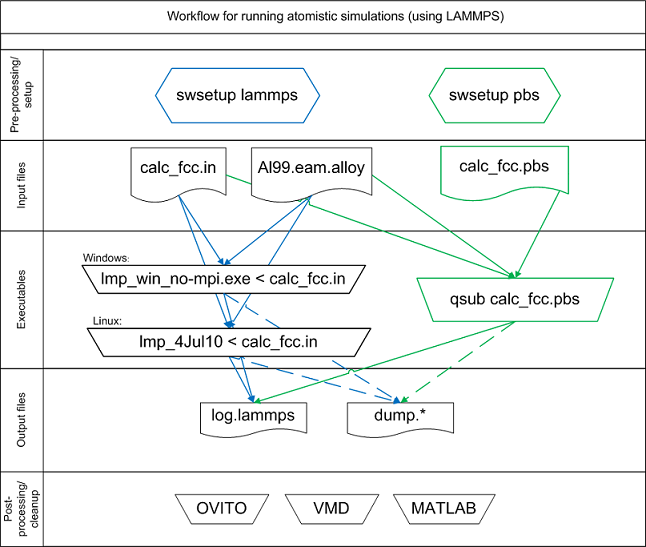
\includegraphics[height=2.50in,width=3.0in, viewport=0 0 646 547,clip]{Lammps_workflow.png}
\caption{\fontsize{6.2pt}{5.2pt}\selectfont{\textrm{The general workflow for running molecular dynamics simulations using LAMMPS.}}}%(与文献\cite{EPJB33-47_2003}图1对比)
\label{General_Workflow}
\end{figure}
}

\frame
{
	\frametitle{\textrm{LAMMPS}的输入参数说明}
	{\fontsize{7.5pt}{5.0pt}\selectfont{
%\verbatiminput{Figures/Lammps_in_lj.txt} %为保险:~选用文件名绝对路径
\verbatiminput{Figures/Lammps_tutorial-01-in_01.txt} %为保险:~选用文件名绝对路径
}
\begin{itemize}
	\item \textcolor{cyan}{\textit{\#}}~开头的部分表示注释,\textrm{LAMMPS}不作任何处理
\end{itemize}
}
\vskip 5pt
%\textrm{LAMMPS}模拟的初始化
{\fontsize{7.5pt}{5.0pt}\selectfont{
%\verbatiminput{Figures/Lammps_in_lj.txt} %为保险:~选用文件名绝对路径
\verbatiminput{Figures/Lammps_tutorial-01-in_02.txt} %为保险:~选用文件名绝对路径
\begin{itemize}
	\item \textcolor{cyan}{\textit{clear}}:~清除全部内存信息
	\item \textcolor{cyan}{\textit{unit}}:~设定模拟的单位~ (\textcolor{blue}{\textrm{metal}}~表示选择\textrm{\AA}和\textrm{eV}为单位)
	\item \textcolor{cyan}{\textit{dimension}}:~设定模拟维度~:~\textcolor{blue}{\textrm{3}}~表示三维模拟
	\item \textcolor{cyan}{\textit{boundary}}~\textcolor{blue}{\textrm{p~p~p}}:~表示在$x$-,$y$-,$z$-方向采用周期性边界条件
		\begin{itemize}
{\fontsize{6.2pt}{5.0pt}\selectfont{
			\item \textrm{p}:~周期性边界条件\textrm{(periodic)}
			\item \textrm{f}:~非周期性固定边界条件\textrm{(fixed)}
			\item \textrm{s}:~非周期性包覆边界条件\textrm{(shrink-wrapped)}
			\item \textrm{m}:~非周期性包覆最小值边界条件\textrm{(minimum value)}}}
		\end{itemize}
\end{itemize}
}}
}

\frame
{
	\frametitle{\textrm{LAMMPS}的输入参数说明}
	{\fontsize{7.5pt}{5.0pt}\selectfont{
\begin{itemize}
	\item \textcolor{cyan}{\textit{atom\_style}}:~设置计算粒子类型~:~\textcolor{blue}{\textrm{atomic}}表示普通原子类型
		\vskip 4pt
		在反应力场计算中,\textcolor{cyan}{\textit{atom\_style}}选用\textcolor{blue}{\textrm{charge}},而\textcolor{cyan}{\textit{units}}选用\textcolor{blue}{\textrm{full}},即反应力场中需要考虑电荷平衡问题
	\item \textcolor{cyan}{\textit{atom\_modify}}:~\textcolor{blue}{\textrm{map~array}}:~表示设置和定义某些存储原子的属性
	\vskip 4pt
	\textcolor{purple}{语法规则}:~\textcolor{cyan}{\textit{atom\_modify}}:~\textcolor{blue}{\textrm{keyword~value}}
	\vskip 3pt
	\textrm{keyword}:~\textrm{\textcolor{blue}{id}~/~\textcolor{blue}{map}~/~\textcolor{blue}{first}}
		\begin{itemize}
{\fontsize{6.2pt}{5.0pt}\selectfont{
\item \textcolor{blue}{\textrm{id~value}}=\textrm{yes~or~no}:~设置是否储存每一个原子的\textrm{ID}(序号) 默认为~\textrm{yes}
\item \textcolor{blue}{\textrm{map~value}}=\textrm{yes~or~array~or~hash}:~设置如何在需要时具有特定\textrm{ID}的原子被发现(\textrm{array}~比\textrm{hash}~快)
\item \textcolor{blue}{\textrm{id~value}}=\textrm{group~ID}:~\textrm{group~ID}~原子首先出现在内部原子列表中的组}}
		\end{itemize}
		\end{itemize}
	}}
}

\frame
{
	\frametitle{\textrm{LAMMPS}的输入参数说明}
	{\fontsize{7.5pt}{5.0pt}\selectfont{
%\verbatiminput{Figures/Lammps_in_lj.txt} %为保险:~选用文件名绝对路径
\verbatiminput{Figures/Lammps_tutorial-01-in_03.txt} %为保险:~选用文件名绝对路径
}
\begin{itemize}
	\item \textcolor{cyan}{\textit{lattice}}:~设定晶格信息~(可选择的晶格类型有\textrm{sc, fcc, bcc, hcp, diamond}等)、\\
		晶格常数(数值\textrm{4})、晶格矢量方向等
	\item \textcolor{cyan}{\textit{region}}:~设定模拟的原胞,此处设定模拟的名为\textcolor{blue}{\textrm{box}}的\textrm{block}(可以理解为原胞)采用晶格单位,并要求\textrm{box}每个方向的大小取为一个晶格常数
	\item \textcolor{cyan}{\textit{create\_box}}:~使用\textcolor{cyan}{\textit{region}}确定的参数构建模拟的\textrm{box},数量为\textcolor{red}{1个}
	\item \textcolor{cyan}{\textit{replicate}}:~设定每个方向上重复的元胞数目
\end{itemize}
}
%\textrm{LAMMPS}模拟的初始化
{\fontsize{7.5pt}{5.0pt}\selectfont{
%\verbatiminput{Figures/Lammps_in_lj.txt} %为保险:~选用文件名绝对路径
\verbatiminput{Figures/Lammps_tutorial-01-in_04.txt} %为保险:~选用文件名绝对路径
}
\begin{itemize}
	\item \textcolor{cyan}{\textit{pair\_style}}:~设定原子间相互作用(力场)类型,此处势函数的形式为~\textcolor{blue}{\textrm{eam/alloy}}
	\item \textcolor{cyan}{\textit{pair\_coeff}}~\textcolor{blue}{\textrm{$\ast$~$\ast$~Al99.eam.alloy~Al}}:~设定相互作用势(力场)的系数\\
		{\fontsize{6.2pt}{5.2pt}\selectfont{\textcolor{magenta}{势函数(力场)的扩展名提示的是使用相互作用的类型}~\textrm{(eam.alloy~=~eam/alloy)}}}
	\item \textcolor{cyan}{\textit{neighbor}}:~设置表面距离
	\item \textcolor{cyan}{\textit{neigh\_modify}}:~设置原子运动
\end{itemize}
}
}

\frame
{
	\frametitle{\textrm{LAMMPS}的输入参数说明}
	{\fontsize{7.5pt}{5.0pt}\selectfont{
%\verbatiminput{Figures/Lammps_in_lj.txt} %为保险:~选用文件名绝对路径
\verbatiminput{Figures/Lammps_tutorial-01-in_05.txt} %为保险:~选用文件名绝对路径
}
\begin{itemize}
	\item \textcolor{cyan}{\textit{compute}}:~定义计算变量:\\
		\begin{enumerate}
{\fontsize{7.5pt}{5.0pt}\selectfont{
\item \textcolor{purple}{变量\textrm{eng}}:~定义为平均每个原子的势能,并且存储在\textrm{ID:~eng}中
\item \textcolor{purple}{变量\textrm{eatom}}:~定义为求和全部\textcolor{purple}{变量\textrm{eng}}的值:~\textcolor{blue}{\textrm{reduce}}~表示减(负)}},对\textrm{eng}求和并存储在\textrm{ID:~eatoms}中
		\end{enumerate}
\end{itemize}
}
}

\frame
{
	\frametitle{\textrm{LAMMPS}的输入参数说明}
%\vskip 5pt
%\textrm{LAMMPS}模拟的初始化
{\fontsize{7.5pt}{5.0pt}\selectfont{
%\verbatiminput{Figures/Lammps_in_lj.txt} %为保险:~选用文件名绝对路径
\verbatiminput{Figures/Lammps_tutorial-01-in_06.txt} %为保险:~选用文件名绝对路径
}
\begin{itemize}
	\item \textcolor{cyan}{\textit{reset\_timestep}}:~重新设定时间模拟步数\footnote{\fontsize{6.2pt}{5.2pt}\selectfont{\textrm{LAMMPS}模拟中,一般需要设置能量最小化、弛豫、数据采集等阶段,不同阶段模拟步数不同。默认情况下,模拟步数是从模拟开始到模拟结束一直累加计算的}}(此处归零:~\textcolor{blue}{\textrm{0}})
	\item \textcolor{cyan}{\textit{fix}}:~设定\textrm{box/relax},能量最小化过程中对模拟盒施外压,各向同性\textrm{(iso)}都弛豫到\textrm{0.0~Pa}:~\textcolor{blue}{\textrm{vmax}}:~正压压缩,负压膨胀
	\item \textcolor{cyan}{\textit{thermo}}:~每运行\textcolor{blue}{10}次在屏幕上输出一次运行结果
	\item \textcolor{cyan}{\textit{thermo\_style}}:~设定屏幕输出信息
	\item \textcolor{cyan}{\textit{min\_style}}:~设定优化算法(最小化算法),\textcolor{blue}{\textrm{cg}}~指定共轭梯度法
	\item \textcolor{cyan}{\textit{minimize}}:~设定开始最小化过程和最小化收敛精度和最大迭代次数:\\
		其中1,3项为能量最小化,2,4项为能量梯度(力)\\
		原胞弛豫的模拟由晶格常数为\textrm{4\AA}到\textrm{4.05\AA}
\end{itemize}
}
}

\frame
{
	\frametitle{\textrm{LAMMPS}的输入参数说明}
	{\fontsize{7.5pt}{5.0pt}\selectfont{
%\verbatiminput{Figures/Lammps_in_lj.txt} %为保险:~选用文件名绝对路径
\verbatiminput{Figures/Lammps_tutorial-01-in_07.txt} %为保险:~选用文件名绝对路径
}
\begin{itemize}
	\item \textcolor{cyan}{\textit{natoms}}:~变量定义所有原子数
	\item \textcolor{cyan}{\textit{teng}}:~变量定义总的势能:~\textcolor{blue}{\textrm{teng=eatoms}}
	\item \textcolor{cyan}{\textit{length}}:~变量定义模拟原胞长度:~\textcolor{blue}{\textrm{length=lx}}(模拟盒$x$方向为例)
	\item \textcolor{cyan}{\textit{ecoh}}:~变量定义内聚能:~\textcolor{blue}{\textrm{ecoh=v\_teng/v\_natoms}}\footnote{\fontsize{6.2pt}{5.2pt}\selectfont{同一语句中出现多个变量引用时用\textrm{\textcolor{red}{v}\_variable}表示}}
\end{itemize}}
%\textrm{LAMMPS}模拟的初始化
{\fontsize{7.5pt}{5.0pt}\selectfont{
%\verbatiminput{Figures/Lammps_in_lj.txt} %为保险:~选用文件名绝对路径
\verbatiminput{Figures/Lammps_tutorial-01-in_08.txt} %为保险:~选用文件名绝对路径
}
\begin{itemize}
	\item 设定屏幕输出和\textrm{log}文件的输出变量
	\item \textcolor{red}{\$\{\}}表示定义变量的引用
\end{itemize}
}
}

%\frame[allowframebreaks]
%{
%	\frametitle{\textrm{LAMMPS}的输入文件}
%\fontsize{6.0pt}{5.0pt}\selectfont{
%%\verbatiminput{Figures/Lammps_in_lj.txt} %为保险:~选用文件名绝对路径
%\verbatiminput{Figures/Lammps_tutorial-01-Lammps-in.txt} %为保险:~选用文件名绝对路径
%}
%}
%
\frame
{
	\frametitle{\textrm{LAMMPS}的输出结果}
	\textrm{LAMMPS}执行命令:
	\vskip 5pt
	\textcolor{blue}{lmp}~\textcolor{magenta}{-in}~calc\_fcc.in
	\vskip 5pt
\begin{figure}[h!]
\centering
\vskip -5pt
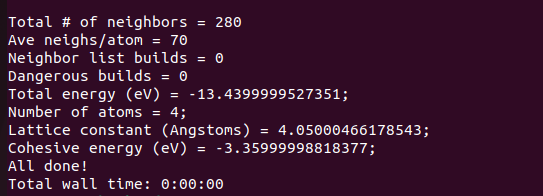
\includegraphics[height=1.50in,width=4.0in, viewport=0 0 543 196,clip]{Lammps_output.png}
\caption{\fontsize{6.2pt}{5.2pt}\selectfont{\textrm{The end of the logfile/screen output using LAMMPS.}}}%(与文献\cite{EPJB33-47_2003}图1对比)
\label{LAMMPS_output}
\end{figure}
}

\subsection{状态方程}
\frame[allowframebreaks]
{
	\frametitle{\textrm{LAMMPS}的输入文件}
	{\fontsize{6.0pt}{5.0pt}\selectfont{
%\verbatiminput{Figures/Lammps_in_lj.txt} %为保险:~选用文件名绝对路径
\verbatiminput{Figures/Lammps_tutorial-02-in.txt} %为保险:~选用文件名绝对路径
}}
	\textrm{LAMMPS}执行命令:
	\vskip 5pt
	\textcolor{blue}{lmp}~\textcolor{magenta}{-in}~calc\_fcc.in~\textcolor{red}{-var~latconst~4}
}

\frame[allowframebreaks]
{
	\frametitle{\textrm{LAMMPS}的输入文件:~基于\textrm{Matlab}的执行}
	{\fontsize{6.0pt}{5.0pt}\selectfont{
%\verbatiminput{Figures/Lammps_in_lj.txt} %为保险:~选用文件名绝对路径
\verbatiminput{Figures/Lammps_tutorial-02-Lammps-in.txt} %为保险:~选用文件名绝对路径
}}
}

\frame[allowframebreaks]
{
	\frametitle{\textrm{LAMMPS}的输入文件:~基于\textrm{Matlab}的执行}
	{\fontsize{6.0pt}{5.0pt}\selectfont{
%\verbatiminput{Figures/Lammps_in_lj.txt} %为保险:~选用文件名绝对路径
\verbatiminput{Figures/Lammps_tutorial-02-Matlab-in.txt} %为保险:~选用文件名绝对路径
}}
}

\frame[allowframebreaks]
{
	\frametitle{\textrm{LAMMPS}的输入文件:~基于\textrm{Python}的执行}
	{\fontsize{6.0pt}{5.0pt}\selectfont{
%\verbatiminput{Figures/Lammps_in_lj.txt} %为保险:~选用文件名绝对路径
\verbatiminput{Figures/Lammps_tutorial-02-Python-in1.txt} %为保险:~选用文件名绝对路径
}}
}

\frame[allowframebreaks]
{
	\frametitle{\textrm{LAMMPS}的输入文件:~基于\textrm{Python}的执行}
	{\fontsize{6.0pt}{5.0pt}\selectfont{
%\verbatiminput{Figures/Lammps_in_lj.txt} %为保险:~选用文件名绝对路径
\verbatiminput{Figures/Lammps_tutorial-02-Python-in2.txt} %为保险:~选用文件名绝对路径
}}
}

\frame
{
	\frametitle{状态方程}
\begin{figure}[h!]
\centering
\vskip -5pt
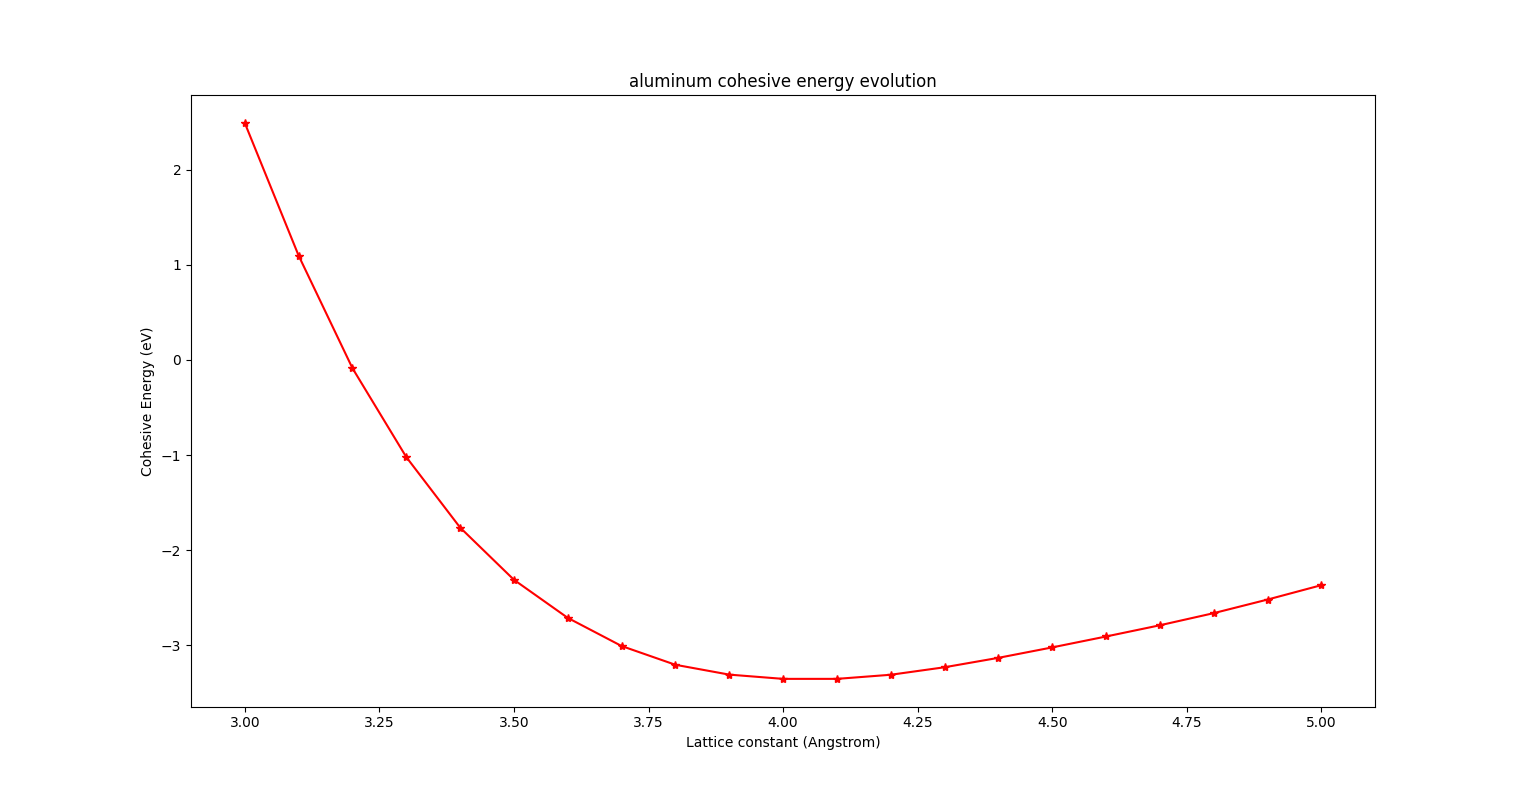
\includegraphics[height=2.50in,width=4.0in, viewport=0 0 1050 554,clip]{Lammps-EOS.png}
\caption{\fontsize{6.2pt}{5.2pt}\selectfont{\textrm{Aluminum cohesive energy evolution.}}}%(与文献\cite{EPJB33-47_2003}图1对比)
\label{LAMMPS_output-EOS}
\end{figure}
}

\subsection{拉伸与压力下的形变模拟}
\frame[allowframebreaks]
{
	\frametitle{\textrm{LAMMPS}的输入文件}
	{\fontsize{6.0pt}{5.0pt}\selectfont{
%\verbatiminput{Figures/Lammps_in_lj.txt} %为保险:~选用文件名绝对路径
\verbatiminput{Figures/Lammps_tutorial-03-Lammps-in.txt} %为保险:~选用文件名绝对路径
}}
}

\frame[allowframebreaks]
{
	\frametitle{\textrm{LAMMPS}的输入文件:~基于\textrm{Matlab}的执行}
	{\fontsize{6.0pt}{5.0pt}\selectfont{
%\verbatiminput{Figures/Lammps_in_lj.txt} %为保险:~选用文件名绝对路径
\verbatiminput{Figures/Lammps_tutorial-03-Matlab-in.txt} %为保险:~选用文件名绝对路径
}}
}

\frame[allowframebreaks]
{
	\frametitle{\textrm{LAMMPS}的输入文件:~基于\textrm{Python}的执行}
	{\fontsize{6.0pt}{5.0pt}\selectfont{
%\verbatiminput{Figures/Lammps_in_lj.txt} %为保险:~选用文件名绝对路径
\verbatiminput{Figures/Lammps_tutorial-03-Python-in.txt} %为保险:~选用文件名绝对路径
}}
}

\frame
{
	\frametitle{应力-应变曲线}
\begin{figure}[h!]
\centering
\vskip -5pt
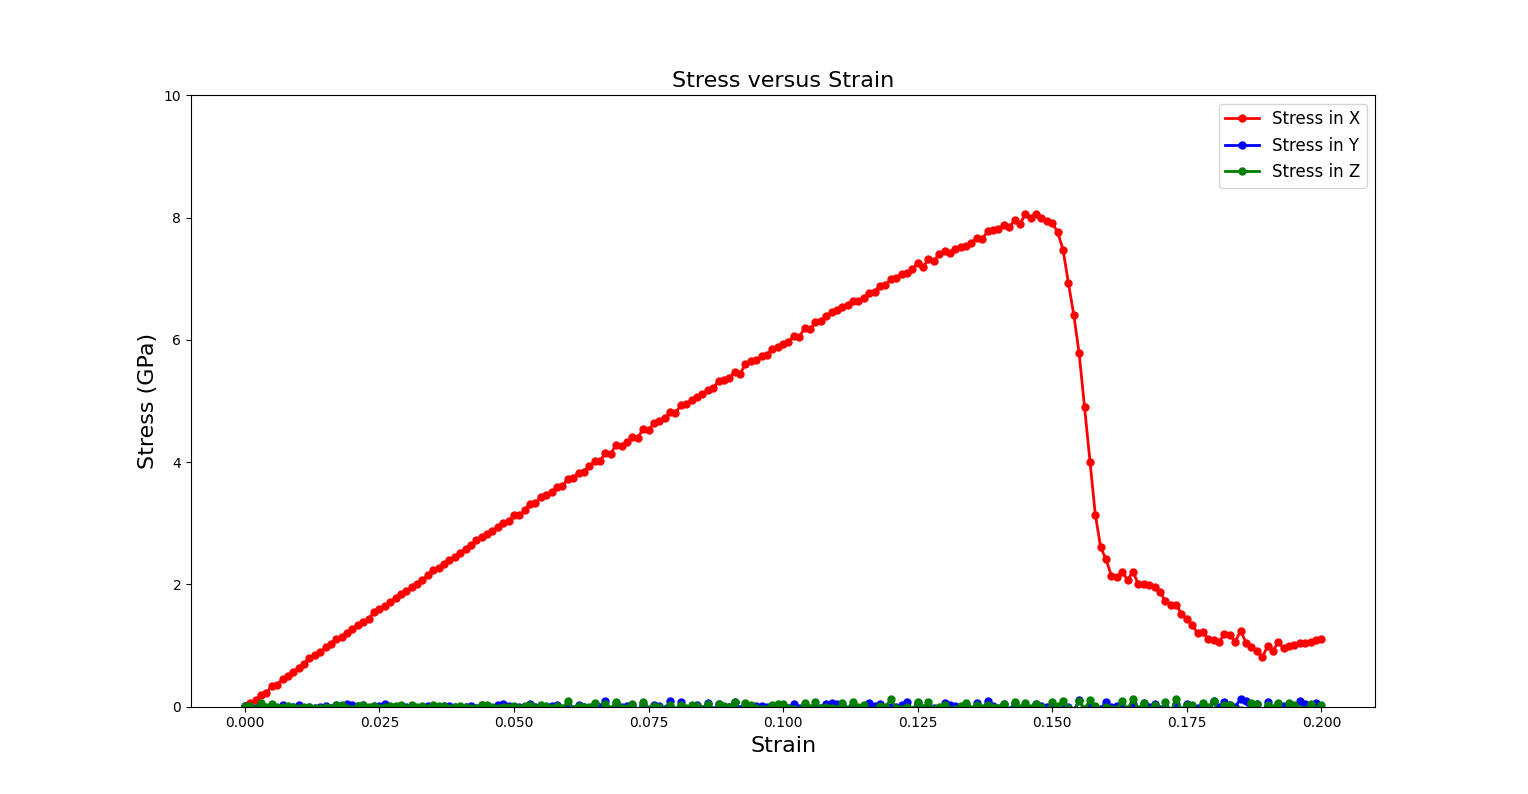
\includegraphics[height=2.20in,width=3.5in, viewport=0 0 1050 554,clip]{Lammps-Stress_Strain.png}
\caption{\fontsize{6.2pt}{5.2pt}\selectfont{\textrm{Stress-strain curve for uniaxial tensile loading of single crystal aluminum in the <100> loading direction.}}}%(与文献\cite{EPJB33-47_2003}图1对比)
\label{LAMMPS_output-Stress-Strain}
\end{figure}
}

\frame
{
	\frametitle{拉伸载荷}
\begin{figure}[h!]
\centering
\vskip -5pt
\animategraphics[autoplay, loop, height=2.40in, width=2.50in,viewport= 0 0 256 256,clip]{1}{Figures/Lammps-simulation-cell-in-tension-}{0}{81}
\caption{\fontsize{6.2pt}{5.2pt}\selectfont{\textrm{Tensile Loading of an Aluminum Single Crystal..}}}%(与文献\cite{EPJB33-47_2003}图1对比)
\label{LAMMPS_Tensile-Loading}
\end{figure}
}

\frame[allowframebreaks]
{
	\frametitle{\textrm{LAMMPS}的输入文件}
	{\fontsize{6.0pt}{5.0pt}\selectfont{
%\verbatiminput{Figures/Lammps_in_lj.txt} %为保险:~选用文件名绝对路径
\verbatiminput{Figures/Lammps_tutorial-04-Lammps-in.txt} %为保险:~选用文件名绝对路径
}}
}

\frame
{
	\frametitle{应力-应变曲线}
\begin{figure}[h!]
\centering
\vskip -5pt
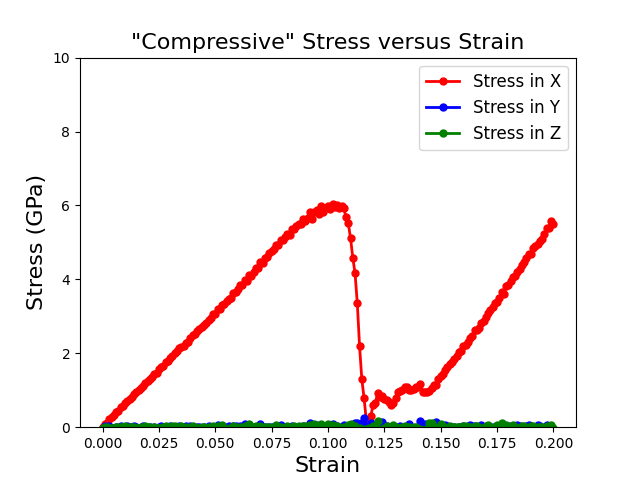
\includegraphics[height=2.40in,width=3.0in, viewport=0 0 450 354,clip]{Lammps-Compressive-Stress_Strain.png}
\caption{\fontsize{6.2pt}{5.2pt}\selectfont{\textrm{Compressive Stress-strain curve for uniaxial compression loading of single crystal aluminum in the <100> loading direction.}}}%(与文献\cite{EPJB33-47_2003}图1对比)
\label{LAMMPS_output-Stress-Strain}
\end{figure}
}

\frame
{
	\frametitle{压缩载荷}
\begin{figure}[h!]
\centering
\vskip -5pt
\animategraphics[autoplay, loop, height=2.40in, width=2.50in,viewport= 0 0 256 256,clip]{1}{Figures/Lammps-simulation-cell-in-compression-}{0}{80}
\caption{\fontsize{6.2pt}{5.2pt}\selectfont{\textrm{Compression Loading of an Aluminum Single Crystal..}}}%(与文献\cite{EPJB33-47_2003}图1对比)
\label{LAMMPS_Compression-Loading}
\end{figure}
}

\subsection{模拟晶界的形成}
\frame[allowframebreaks]
{
	\frametitle{\textrm{LAMMPS}的输入文件}
	{\fontsize{6.0pt}{5.0pt}\selectfont{
%\verbatiminput{Figures/Lammps_in_lj.txt} %为保险:~选用文件名绝对路径
\verbatiminput{Figures/Lammps_tutorial-05-Lammps-in.txt} %为保险:~选用文件名绝对路径
}}
}

\subsection{拉伸晶界直至断裂}
\frame[allowframebreaks]
{
	\frametitle{\textrm{LAMMPS}的输入文件}
	{\fontsize{6.0pt}{5.0pt}\selectfont{
%\verbatiminput{Figures/Lammps_in_lj.txt} %为保险:~选用文件名绝对路径
\verbatiminput{Figures/Lammps_tutorial-06-Lammps-in.txt} %为保险:~选用文件名绝对路径
}}
}

\subsection{铁的对称倾转晶界断裂的原子模拟}
\frame[allowframebreaks]
{
	\frametitle{\textrm{LAMMPS}的输入文件}
	{\fontsize{6.0pt}{5.0pt}\selectfont{
%\verbatiminput{Figures/Lammps_in_lj.txt} %为保险:~选用文件名绝对路径
\verbatiminput{Figures/Lammps_tutorial-07-Lammps-in.txt} %为保险:~选用文件名绝对路径
}}
}

\frame[allowframebreaks]
{
	\frametitle{\textrm{LAMMPS}的\textrm{data}文件}
	{\fontsize{6.0pt}{5.0pt}\selectfont{
%\verbatiminput{Figures/Lammps_in_lj.txt} %为保险:~选用文件名绝对路径
\verbatiminput{Figures/Lammps_tutorial-07-Lammps-data.txt} %为保险:~选用文件名绝对路径
}}
}

\subsection{聚合物链行为模拟}
\frame[allowframebreaks]
{
	\frametitle{\textrm{LAMMPS}的\textrm{data}文件}
	{\fontsize{6.0pt}{5.0pt}\selectfont{
%\verbatiminput{Figures/Lammps_in_lj.txt} %为保险:~选用文件名绝对路径
\verbatiminput{Figures/Lammps_tutorial-08-Lammps-data.txt} %为保险:~选用文件名绝对路径
}}
}

\frame
{
	\frametitle{\textrm{LAMMPS}中的键角与二面角}
\begin{figure}[h!]
\centering
\vskip -5pt
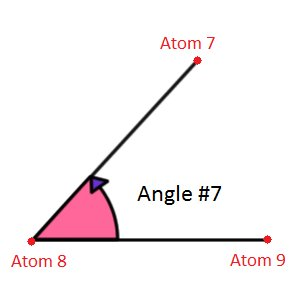
\includegraphics[height=1.70in,width=1.9in, viewport=0 0 320 280,clip]{Lammps-Angles_between_atoms.jpeg}
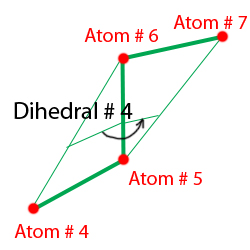
\includegraphics[height=1.70in,width=1.9in, viewport=0 0 280 250,clip]{Lammps-Dihedral_angles_between_atoms.jpeg}
\caption{\fontsize{6.2pt}{5.2pt}\selectfont{\textrm{A schematic of angles~(left) and dihedral angles~(right) between atoms defined in LAMMPS.}}}%(与文献\cite{EPJB33-47_2003}图1对比)
\label{LAMMPS_Angle-and-Dihedral_angle}
\end{figure}
}

\frame[allowframebreaks]
{
	\frametitle{\textrm{LAMMPS}的输入文件}
	{\fontsize{6.0pt}{5.0pt}\selectfont{
%\verbatiminput{Figures/Lammps_in_lj.txt} %为保险:~选用文件名绝对路径
\verbatiminput{Figures/Lammps_tutorial-08-Lammps-in.txt} %为保险:~选用文件名绝对路径
}}
}

%\vskip 5pt
\section{模型算例}
\subsection{金纳米线的断裂模拟}
\frame[allowframebreaks]
{
	\frametitle{\textrm{LAMMPS}的输入文件}
	{\fontsize{6.0pt}{5.0pt}\selectfont{
\verbatiminput{Figures/Lammps_tutorial-11-in.txt} %为保险:~选用文件名绝对路径
}}
}

\frame
{
	\frametitle{金纳米线的断裂模拟}
\begin{figure}[h!]
\centering
\vskip -5pt
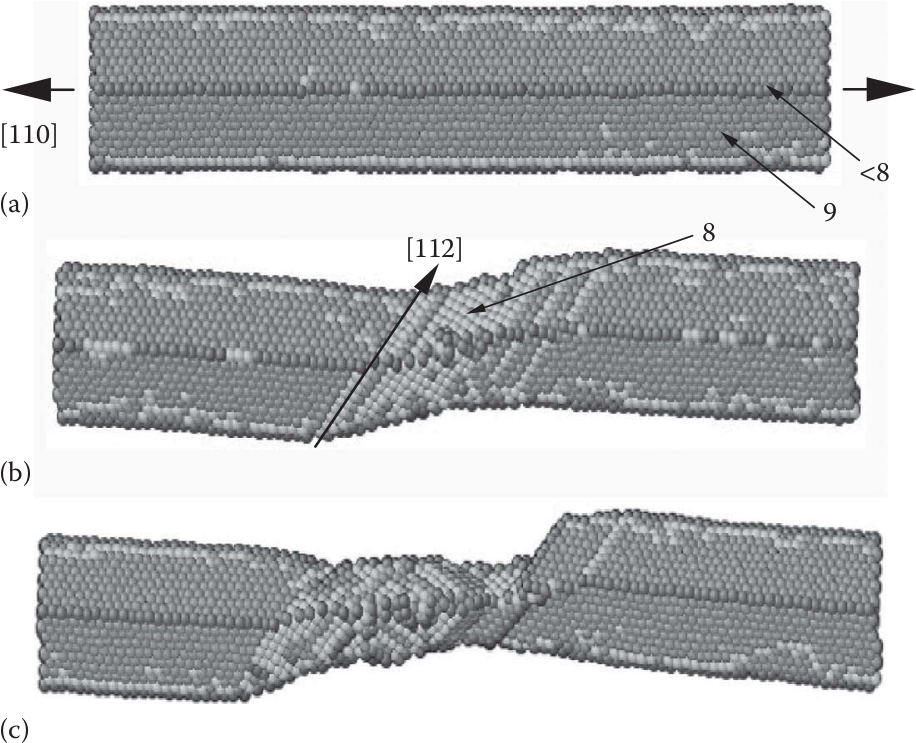
\includegraphics[height=2.40in,width=4.0in, viewport=0 0 940 740,clip]{Lammps_tutorial-11-tensile_loading.png}
\caption{\fontsize{6.2pt}{5.2pt}\selectfont{\textrm{Deformation behavior of an Au nanowire during tensile loading. Timestep=0~(a), 150,000~(b), 282,000~(c).}}}%(与文献\cite{EPJB33-47_2003}图1对比)
\label{LAMMPS_Au-nanowire}
\end{figure}
}

\subsection{纳米水粒滴被石墨烯纳米带的自发包裹}
\frame[allowframebreaks]
{
	\frametitle{\textrm{LAMMPS}的输入文件}
	{\fontsize{6.0pt}{5.0pt}\selectfont{
\verbatiminput{Figures/Lammps_tutorial-12-in.txt} %为保险:~选用文件名绝对路径
}}
}

\frame[allowframebreaks]
{
	\frametitle{\textrm{LAMMPS}的\textrm{data}文件}
	{\fontsize{6.0pt}{5.0pt}\selectfont{
%\verbatiminput{Figures/Lammps_in_lj.txt} %为保险:~选用文件名绝对路径
\verbatiminput{Figures/Lammps_tutorial-12-data.txt} %为保险:~选用文件名绝对路径
}}
}

\frame
{
	\frametitle{纳米水粒滴的自发包裹}
\begin{figure}[h!]
\centering
\vskip -5pt
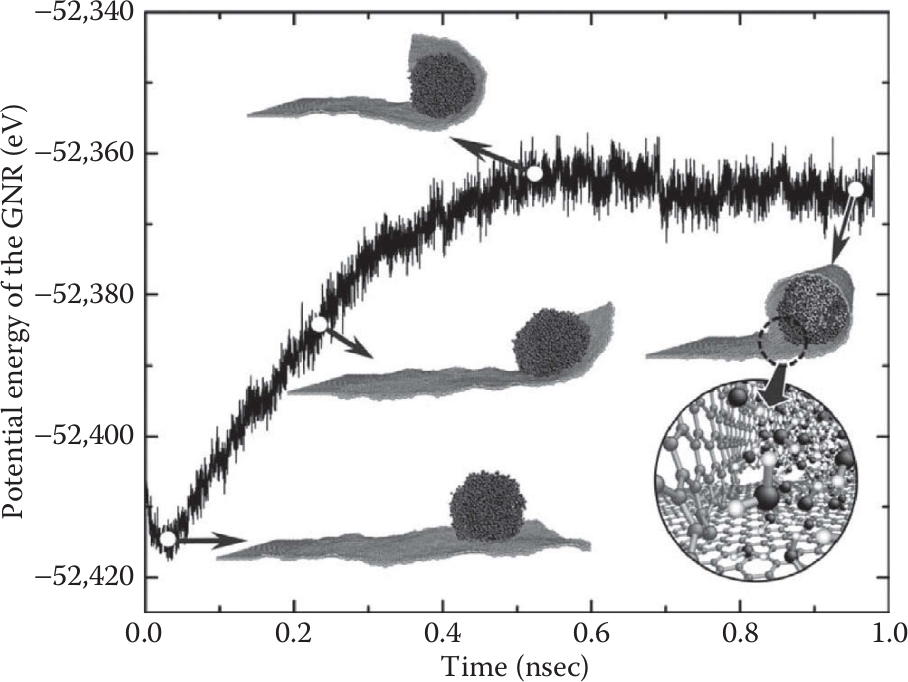
\includegraphics[height=2.40in,width=3.1in, viewport=0 0 940 700,clip]{Lammps_tutorial-12-spontaneous_wrapping.png}
\caption{\fontsize{6.2pt}{5.2pt}\selectfont{\textrm{Spontaneous wrapping of a water nanodroplet by the GNR.}}}%(与文献\cite{EPJB33-47_2003}图1对比)
\label{LAMMPS_water-nanodroplet-spontaneous-wrapping-GNR}
\end{figure}
}

\subsection{碳纳米管的拉伸}
\frame[allowframebreaks]
{
	\frametitle{\textrm{LAMMPS}的输入文件}
	{\fontsize{6.0pt}{5.0pt}\selectfont{
\verbatiminput{Figures/Lammps_tutorial-13-in.txt} %为保险:~选用文件名绝对路径
}}
}

\frame[allowframebreaks]
{
	\frametitle{\textrm{LAMMPS}的\textrm{data}文件}
	{\fontsize{6.0pt}{5.0pt}\selectfont{
%\verbatiminput{Figures/Lammps_in_lj.txt} %为保险:~选用文件名绝对路径
\verbatiminput{Figures/Lammps_tutorial-13-data.txt} %为保险:~选用文件名绝对路径
}}
}

\frame
{
	\frametitle{碳纳米管的断裂模拟}
\begin{figure}[h!]
\centering
\vskip -5pt
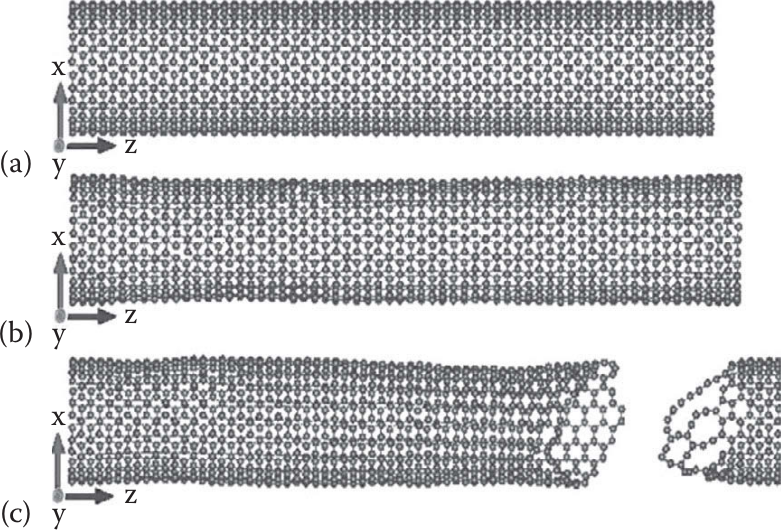
\includegraphics[height=2.40in,width=3.5in, viewport=0 0 820 520,clip]{Lammps_tutorial-13-Fracture_of_a_CNT_under_tension.png}
\caption{\fontsize{6.2pt}{5.2pt}\selectfont{\textrm{Fracture of a CNT under tension at timesteps of 0~(a), 20,000~(b), 40,000~(c).}}}%(与文献\cite{EPJB33-47_2003}图1对比)
\label{LAMMPS_Frcture-of-CNT-under_ternsion}
\end{figure}
}

\frame
{
	\frametitle{拉伸条件下碳纳米管的应力-应变}
\begin{figure}[h!]
\centering
\vskip -5pt
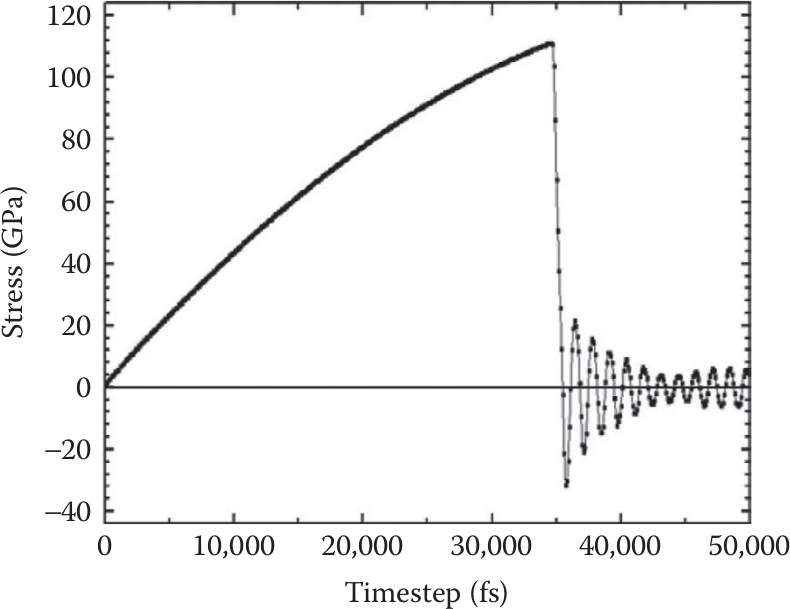
\includegraphics[height=2.40in,width=3.1in, viewport=0 0 820 620,clip]{Lammps_tutorial-13-Stress_strain-curve-of-a-CNT_under_tension.png}
\caption{\fontsize{6.2pt}{5.2pt}\selectfont{\textrm{Stress–strain curve of a CNT under tension.}}}%(与文献\cite{EPJB33-47_2003}图1对比)
\label{LAMMPS_Stress_strain-of-CNT_under_tension}
\end{figure}
}

\subsection{硅柱的拉伸裂纹}
\frame[allowframebreaks]
{
	\frametitle{\textrm{LAMMPS}的输入文件}
	{\fontsize{6.0pt}{5.0pt}\selectfont{
\verbatiminput{Figures/Lammps_tutorial-14-in.txt} %为保险:~选用文件名绝对路径
}}
}

\frame
{
	\frametitle{硅柱的断纹模拟}
\begin{figure}[h!]
\centering
\vskip -15pt
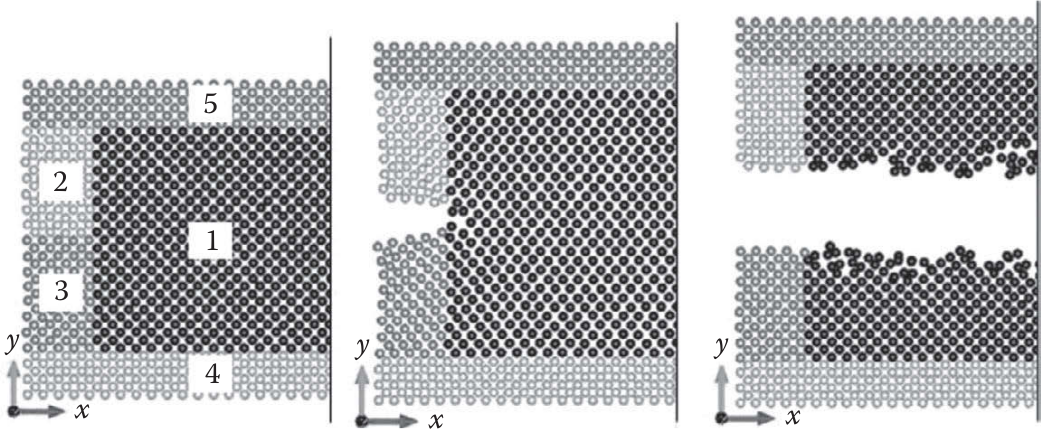
\includegraphics[height=2.10in,width=4.0in, viewport=0 0 1050 500,clip]{Lammps_tutorial-14-Si_crack-initiating-block_under_tension.png}
\caption{\fontsize{6.2pt}{5.2pt}\selectfont{\textrm{Si bar with a small crack-initiating block under tension: at timesteps of 0~(a), 15,000~(b), 25,000~(c).}}}%(与文献\cite{EPJB33-47_2003}图1对比)
\label{LAMMPS_Si_bar-Crack-initiating_block_under_tension}
\end{figure}
}

\frame
{
	\frametitle{拉伸裂纹与硅柱的应力-应变}
\begin{figure}[h!]
\centering
\vskip -5pt
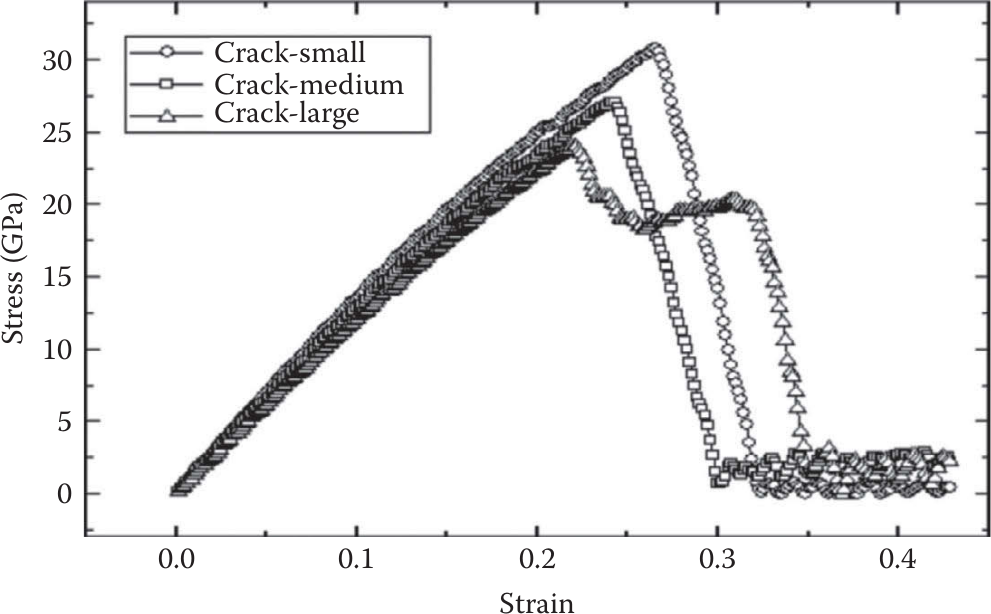
\includegraphics[height=2.40in,width=3.5in, viewport=0 0 1000 620,clip]{Lammps_tutorial-14-Stress_strain-curves-Si_crack-initiating-block_under_tension.png}
\caption{\fontsize{6.2pt}{5.2pt}\selectfont{\textrm{Stress–strain curve of Si bars with various initial crack sizes.}}}%(与文献\cite{EPJB33-47_2003}图1对比)
\label{LAMMPS_Stress_strain-of-Si_bar-with-various_initial_crack_sizes}
\end{figure}
}

\subsection{硅-碳纳米管复合材料的拉伸}
\frame
{
	\frametitle{硅-碳纳米管复合材料的设计}
\begin{figure}[h!]
\centering
\vskip -8pt
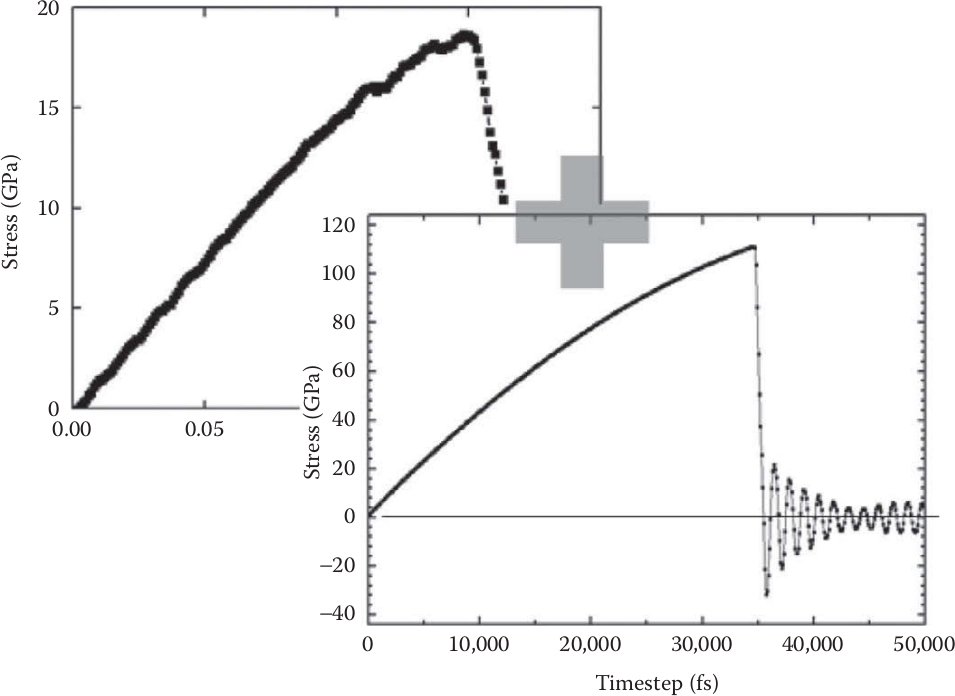
\includegraphics[height=2.70in,width=3.6in, viewport=0 0 960 700,clip]{Lammps_tutorial-15-design_concept-for-the-Si-CNT.png}
\caption{\fontsize{6.2pt}{5.2pt}\selectfont{\textrm{Design concept for the Si–CNT composite system.}}}%(与文献\cite{EPJB33-47_2003}图1对比)
\label{LAMMPS_Design_concept-for-Si_CNT.}
\end{figure}
}

\frame[allowframebreaks]
{
	\frametitle{\textrm{LAMMPS}的输入文件}
	{\fontsize{6.0pt}{5.0pt}\selectfont{
\verbatiminput{Figures/Lammps_tutorial-15-in.txt} %为保险:~选用文件名绝对路径
}}
}

\frame
{
	\frametitle{硅-碳纳米管复合材料的初始结构}
\begin{figure}[h!]
\centering
\vskip -10pt
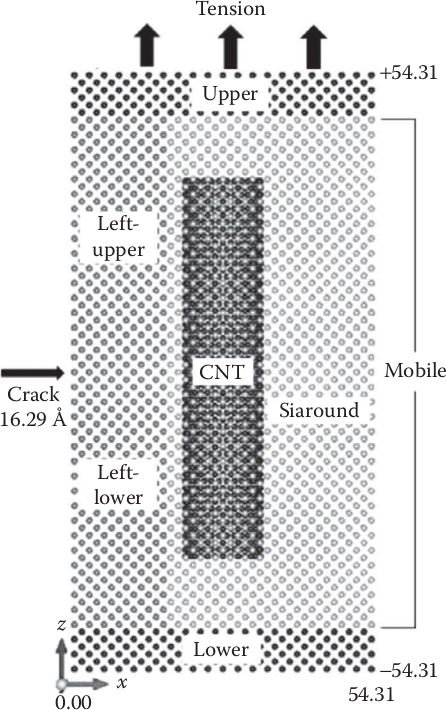
\includegraphics[height=2.70in,width=2.1in, viewport=0 0 500 720,clip]{Lammps_tutorial-15-starting_structure-for-the-Si-CNT.png}
\caption{\fontsize{6.2pt}{5.2pt}\selectfont{\textrm{Starting structure of the Si–CNT composite system.}}}%(与文献\cite{EPJB33-47_2003}图1对比)
\label{LAMMPS_Starting-structure-of-Si_CNT.}
\end{figure}
}

\frame[allowframebreaks]
{
	\frametitle{\textrm{LAMMPS}的\textrm{data}文件}
	{\fontsize{6.0pt}{5.0pt}\selectfont{
%\verbatiminput{Figures/Lammps_in_lj.txt} %为保险:~选用文件名绝对路径
\verbatiminput{Figures/Lammps_tutorial-15-data.txt} %为保险:~选用文件名绝对路径
}}
}

\frame
{
	\frametitle{硅-碳纳米管复合材料的原子间相互作用}
\begin{figure}[h!]
\centering
\vskip -5pt
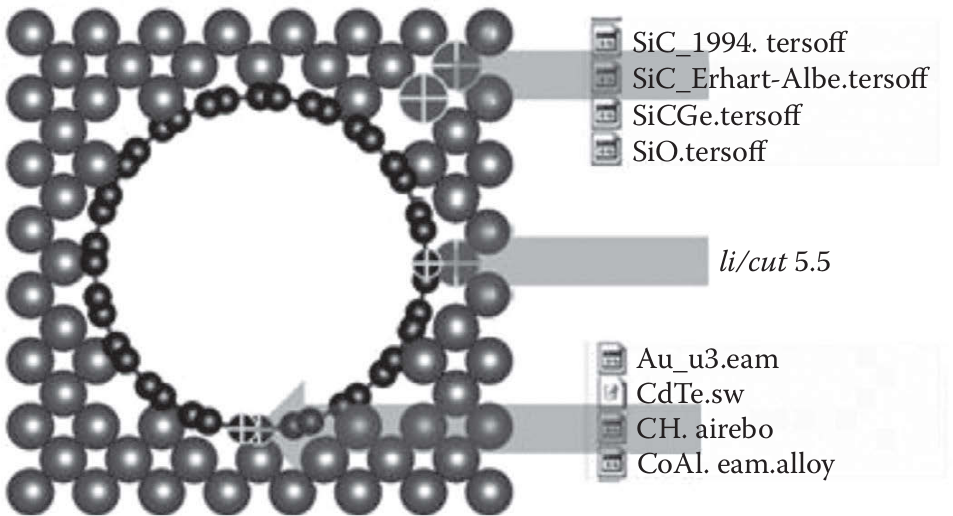
\includegraphics[height=2.40in,width=4.0in, viewport=0 0 940 540,clip]{Lammps_tutorial-15-three_potentials-adopted-for_Si-CNT_and_their-interface.png}
\caption{\fontsize{6.2pt}{5.2pt}\selectfont{\textrm{Three potentials adopted for the study to describe Si, CNT, and their interface.}}}%(与文献\cite{EPJB33-47_2003}图1对比)
\label{LAMMPS_Potential-Si-CNT}
\end{figure}
}

\frame
{
	\frametitle{硅-碳纳米管复合材料的拉伸过程}
\begin{figure}[h!]
\centering
\vskip -10pt
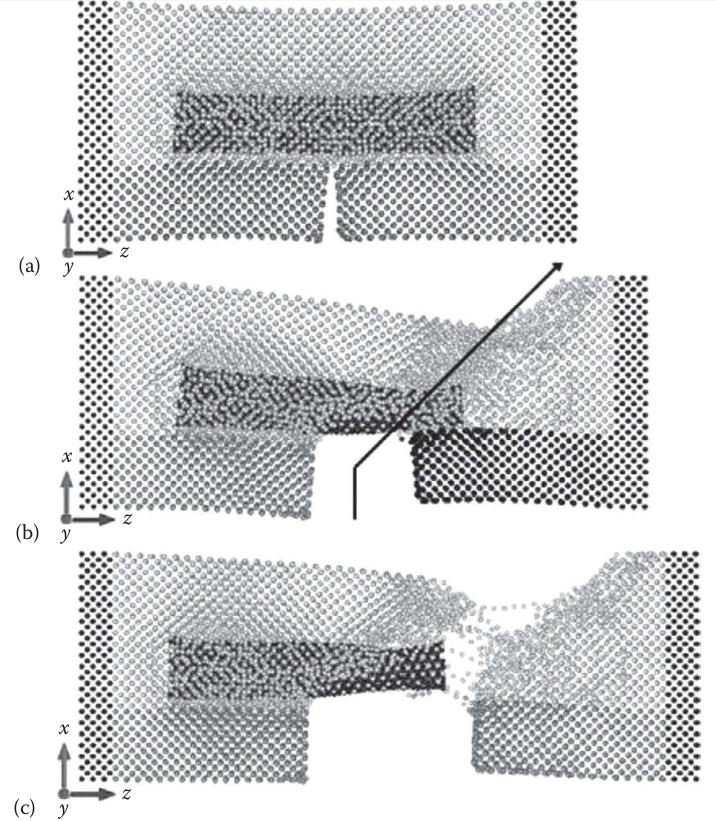
\includegraphics[height=2.60in,width=2.8in, viewport=0 0 770 820,clip]{Lammps_tutorial-15-snapshots_of_the Si-CNT_composite_system_under-tension-for-various-strains.png}
\caption{\fontsize{6.2pt}{5.2pt}\selectfont{\textrm{Snapshots of the Si–CNT composite system with $\varepsilon=0.5\mathrm{eV}$ under tension for various strains:~10.5\%~(a), 31.5\%~(b), 42\%~(c).}}}%(与文献\cite{EPJB33-47_2003}图1对比)
\label{LAMMPS_Si_CNT-under-tension}
\end{figure}
}

\frame
{
	\frametitle{硅-碳纳米管复合材料拉伸的应力-应变}
\begin{figure}[h!]
\centering
\vskip -5pt
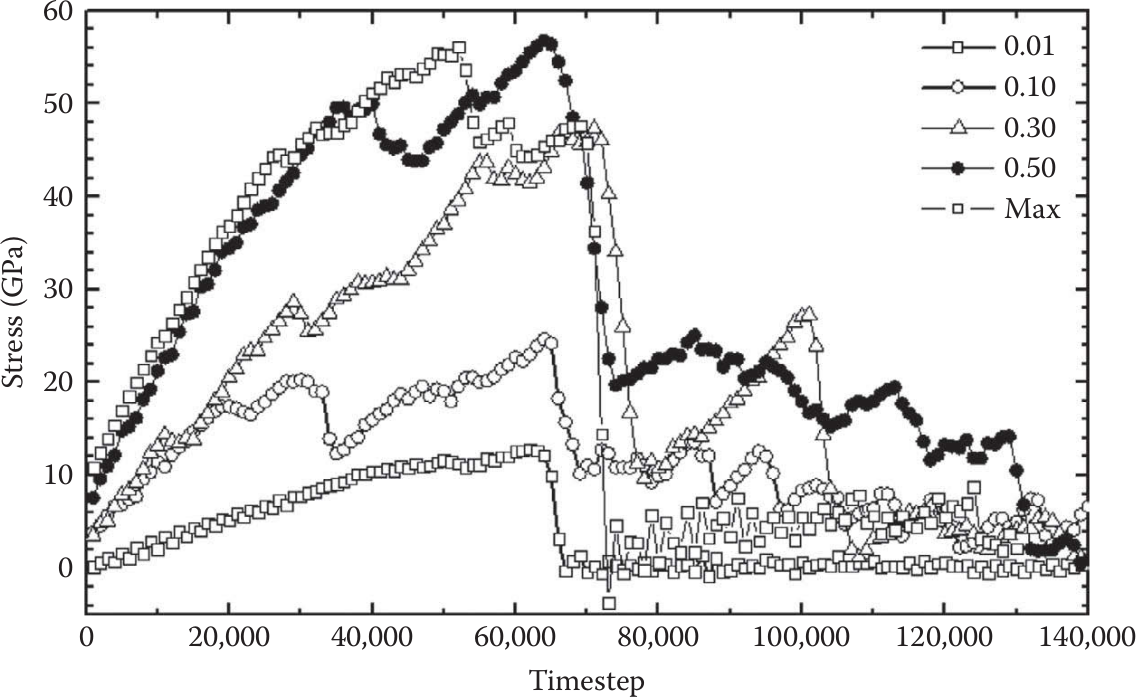
\includegraphics[height=2.42in,width=4.0in, viewport=0 0 1200 730,clip]{Lammps_tutorial-15-Stress_strain-curves-of-the-Si-CNT.png}
\caption{\fontsize{6.2pt}{5.2pt}\selectfont{\textrm{Stress–strain curves of the Si–CNT nanocomposites with various interfacial bonding strengths.}}}%(与文献\cite{EPJB33-47_2003}图1对比)
\label{LAMMPS_Stress-train-curve}
\end{figure}
}

\subsection{$\mathrm{ZrO}_2$-\rm{8}-$\mathrm{Y}_2\mathrm{O}_3$的均方位移}
\frame[allowframebreaks]
{
	\frametitle{\textrm{LAMMPS}的输入文件}
	{\fontsize{6.0pt}{5.0pt}\selectfont{
\verbatiminput{Figures/Lammps_tutorial-16-in.txt} %为保险:~选用文件名绝对路径
}}
}

\frame
{
	\frametitle{$\mathrm{ZrO}_2$-\textrm{8}$\mathrm{Y}_2\mathrm{O}_3$的结构}
\begin{figure}[h!]
\centering
\vskip -5pt
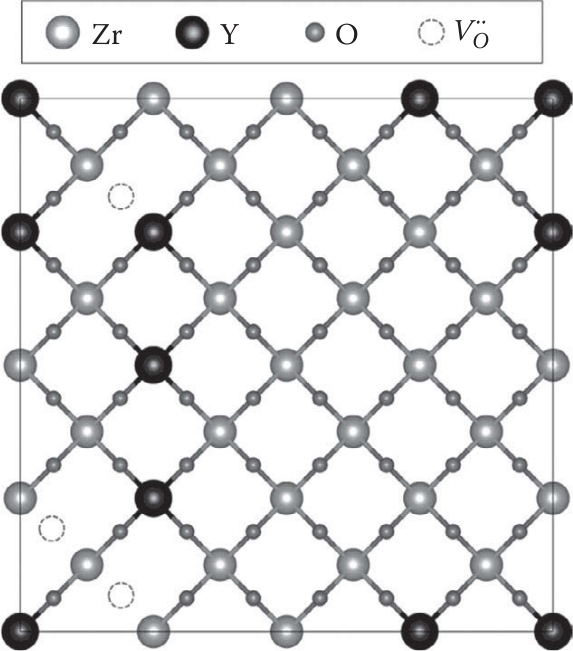
\includegraphics[height=2.40in,width=2.3in, viewport=0 0 640 680,clip]{Lammps_tutorial-16-sliced-structure-of-ZrO2-8Y2O3-system.png}
\caption{\fontsize{6.2pt}{5.2pt}\selectfont{\textrm{Sliced structure of the $\mathrm{ZrO}_2$-8$\mathrm{Y_2O_3}$ system showing a metal ($\mathrm{Zr}$ and $\mathrm{Y}$) layer and an oxygen layer along the [001] direction.}}}%(与文献\cite{EPJB33-47_2003}图1对比)
\label{LAMMPS_slice-structure-of-ZrO2-8Y2O3}
\end{figure}
}

\frame[allowframebreaks]
{
	\frametitle{\textrm{LAMMPS}的\textrm{data}文件}
	{\fontsize{6.0pt}{5.0pt}\selectfont{
%\verbatiminput{Figures/Lammps_in_lj.txt} %为保险:~选用文件名绝对路径
\verbatiminput{Figures/Lammps_tutorial-16-data.txt} %为保险:~选用文件名绝对路径
}}
}

\frame
{
	\frametitle{均方位移\textrm{(Mean-Squared Displacement,MSD)}}
\begin{figure}[h!]
\centering
\vskip -5pt
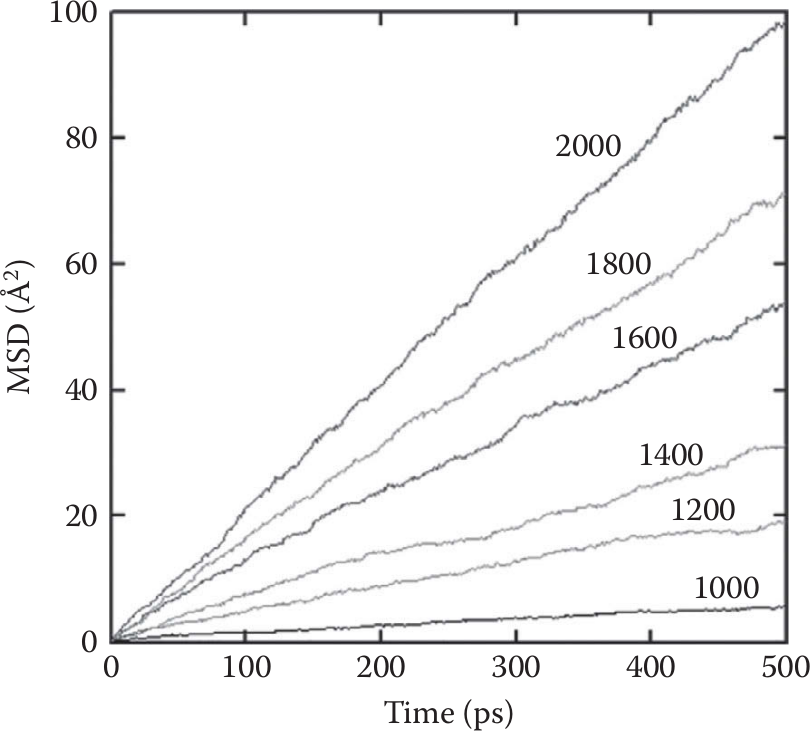
\includegraphics[height=2.50in,width=3.2in, viewport=0 0 850 780,clip]{Lammps_tutorial-16-MSD_plot-with-time_in-the_last_500000-timesteps.png}
\caption{\fontsize{6.2pt}{5.2pt}\selectfont{\textrm{MSD plot with time in the range of the last 500,000 timesteps at various temperatures from 2,000 to 1,000 K.}}}%(与文献\cite{EPJB33-47_2003}图1对比)
\label{LAMMPS_MSD-ZrO2-8Y2O3.}
\end{figure}
}

%------------------------------------------------------------------------Reference----------------------------------------------------------------------------------------------
		\frame[allowframebreaks]
{
\frametitle{主要参考文献}
\begin{thebibliography}{99}
{\tiny
	\bibitem{url_lammps-tutorials}\url{https://github.com/mrkllntschpp/lammps-tutorials}
	\bibitem{J.-G._Lee}\textrm{J.-G. Lee, \textit{Computational Materials Science:~an introduction}}~\textrm{(2nd Edition),~CPC Press}, \textrm{(2017)}
%	\bibitem{url_Atom-Eye}\url{http://li.mit.edu/Archive/Graphics/A/}
		\vskip 5pt \textcolor{blue}{\textrm{LAMMPS}常用的可视化软件}
\bibitem{url_Atom-Eye_download}\url{http://li.mit.edu/Archive/Graphics/A/#download}
%\bibitem{url_ImageJ}\url{https://imagej.net/ij/}
\bibitem{url_ImageJ_download}\url{https://imagej.net/ij/download.html}
\bibitem{url_ovito_download}\url{https://www.ovito.org/os-downloads/}
}
\end{thebibliography}
}
